

\chapter{Introducción} 
\label{cap:intro}


% \todo{Entiendo que quieres comentar la importancia de los gráficos por computador en el mundo actual. Primero te comento errores cometidos y luego te propongo soluciones:
% 1. La generación de imágenes hace referencia solo al proceso de renderizado. El área de conocimiento son los gráficos por computar, estos incluyen animación, modelado, post-proceso.
% 2. El mundo del la generaicón y tratamiento de imagenes es demasiado amplio. Tú deberías centrarlo en el campo del los gráficos 3D (aquellos en los que la imagen generada nos permite de alguna manera (claves perpetúales captar la profundidad))
% 3. Todo el mundo sabe que los gráficos 3D estan tanformando el mundo del ocio (peliculas de animación, videojuegos) y el mundo profesional (por cierto no hablaria del mundo profesional, hablaria de la cientcia, el foramción, analisis de datos, interacción hombre máquina ...). Pero en este párrafo no concretas estas aportaciones. Ocio: ciene y videojuegos, Apredizaje: gamificación, entremiento en entornos seguros. Ciencia: Visualización y análisis de datos.... 
% Solución:
% No hables de los graficos por computador. Tu tesis se enmarca en la RV. La RV utiliza los graficos por computador y muchas otras displinas. 
% Te estoy metiendo comentarios largos por si te pueden ayudar con futuras redacciones. }

Durante los últimos años, el término de \ac{RV} se ha incorporado a nuestro lenguaje cotidiano. Esto es debido a la gran penetración que están teniendo este tipo de sistemas en nuestra vida privada y, cada vez más, en distintos ámbitos profesionales. Se pueden encontrar ejemplos de estas aplicaciones en sectores tan diversos como: el mundo del ocio, donde los videojuegos son el máximo exponente del uso de estas tecnologías; el campo del entrenamiento profesional, en el que la \ac{RV} permite el desarrollo de destrezas no cognitivas en entornos controlados \cite{PATEL2017266.e7}; el ámbito científico, donde estos sistemas facilitan la compresión de datos complejos mediante el uso de entornos inmersos \cite{usher2018}. Dado el gran número de campos de aplicación y de tecnologías utilizadas, no resulta fácil indicar de forma unívoca qué caracteriza una aplicación de \ac{RV}. En la bibliografía, se pueden encontrar distintas definiciones del término:

\begin{center}
    \begin{minipage}{0.9\linewidth}
        %\vspace{5pt}%margen superior de minipage
        {\small
\emph{Virtual reality is a high-end user-computer interface that
involves real-time simulation and interactions through
multiple sensorial channels.}
        }
        \begin{flushright}
            (Burdea y Coiffet, 2003: \cite{burdea2003virtual})
        \end{flushright}
        %\vspace{5pt}%margen inferior de la minipage
    \end{minipage}
    
    \begin{minipage}{0.9\linewidth}
        %\vspace{5pt}%margen superior de minipage
        {\small
\emph{VR is the science and technology required for a user
to feel present, via perceptive, cognitive and functional
immersion and interaction, in a (computer) generated
environment. }
        }
        \begin{flushright}
            (Casarin et al., 2015: \cite{kuntz2015middlevr})
        \end{flushright}
        %\vspace{5pt}%margen inferior de la minipage
    \end{minipage}
    
\end{center}
%
%\todo{1.La realidad virtual no es una subcampo del los graficos por computdor.2.En algún lugar hay que hablar de la multidisciplinaridad de este campo (ingeniería, ciencias de la computación, psicología, graficos por computador...). Puede ir despues de la definición.}
% Este comentario esta para que no sea un parrafo nuevo
Tal y como se desprende de las definiciones anteriores, las aplicaciones \ac{RV} se caracterizan por presentar al usuario un entorno virtual a través de varios canales sensoriales, permitiéndole interactuar con el mismo y generando en él, una sensación de inmersión y presencia \cite{Jerald:2015}. Estos objetivos imprimen a este campo una naturaleza altamente multidisciplinar. La \ac{RV} se asienta en disciplinas como la ingeniería mecánica, los gráficos por computador, la percepción, la computación de altas prestaciones, etcétera. De esta forma, el desarrollo de estas aplicaciones requiere naturalmente de expertos en distintas áreas de conocimiento.  

%\todo{ojo con afirmar cosas que no estan justificadas como "inmersión completa" o "todos los sentidos"}

El auge de la \ac{RV} es evidente, pudiéndose encontrar multitud de aplicaciones en campos tan diversos como el arte, el marketing, la psicología, el diseño y prototipado..., siendo los sectores del entrenamiento de profesionales (de muy diversa naturaleza) y del ocio, en los que más se ha desarrollado.

%\todo{1. Es importante en las 2. 2. En lugar de decir que los entrenadores virtuales son de gran importancia, di que es donde se enmarca este trabajo de tesis.3. Explica las ventajas frente a los métodos clasicos. Es en esta última, donde la \ac{RV} tiene una gran importancia ya que se ha podido comprobar que puede traer grandes beneficios en la enseñanza y aprendizaje utilizando las nuevas tecnologías de manera atractiva frente a los métodos clásicos.}
Esta tesis se centrará en el ámbito de las aplicaciones de \ac{RV} con fines de entrenamiento de profesionales en tareas complejas. En muchas profesiones, existen procesos que requieren destrezas no cognitivas que solo pueden adquirirse mediante la práctica, siendo necesario recurrir a técnicas de entrenamiento alternativas y, especialmente, cuando la actividad entraña un riesgo para el profesional o para terceros. En estos casos, las aplicaciones de \ac{RV} han demostrado  grandes ventajas sobre las técnicas de entrenamiento tradicional~\cite{PATEL2017266.e7}, proporcionando un entorno seguro, repetible y variado en los escenarios donde los usuarios pueden practicar. A pesar de ello, el desarrollo e implantación de estos sistemas no está exento de dificultades. Se deben diseñar (con una correspondiente evaluación a posteriori) de forma que las destrezas que se pretenden adquirir sean transferibles del entorno virtual al mundo real. Además, es importante garantizar que no se adquieran malos hábitos o destrezas solamente válidas en el contexto del simulador.

Dicho esto, uno de los campos donde los entrenadores virtuales han penetrado con más fuerza, es el de la aviación \cite{lee2017flight}. Los simuladores de vuelo son una herramienta esencial que forma parte del currículum de los nuevos pilotos comerciales \cite{piloto}. El objetivo de estas herramientas no es solo de entrenamiento, sino que también proporcionan una plataforma de evaluación.  %\todo{Aaron intenta ser un poco más formal: Concretamente la EASA (poner en tu lista de acrónimos) establece el uso del simulardores de vuelo en curriculum de los futuros pilotos comerciales como un requisito para obtener su licencia}
Concretamente, la \ac{EASA} establece el uso de los simuladores de vuelo en el currículum de los futuros pilotos comerciales como un requisito para obtener su licencia \cite{normativa}.
%\todo{Busca si es por ley y cambia la frase}.

%\todo{Aaron te lo he cambiado para que suene más formal. Cuando metas una frase léelo 2 veces para ver si puede hacer que suene mejor}
Por otra parte, otro campo donde son evidentes los beneficios de la \ac{RV} es  el ámbito médico. Un ejemplo claro son las prácticas quirúrgicas donde se requiere de la manipulación mecánica de estructuras anatómicas. De este modo, el entrenamiento de dichos procedimientos se caracteriza por tener un alto componente práctico, de cara a adquirir las destrezas no cognitivas con las que asegurar que en el futuro se procederá de manera efectiva y segura.
%\del{Por otra parte, en el ámbito médico, la prácticas quirúrgicas requieren de la manipulación se encarga de la curación del paciente mediante la manipulación mecánica de las estructuras anatómicas y por ende su aprendizaje se caracteriza por un gran componente práctico.}
Es por ello que, dado el riesgo que suelen representar este tipo de técnicas para los pacientes, este campo está especialmente interesado en el desarrollo de nuevas metodologías que den la posibilidad de entrenar en entornos seguros, repetibles y variados. Por este motivo, en los últimos años siguen proliferando trabajos académicos que proponen nuevos simuladores médicos de \ac{RV}~\cite{korzeniowski2018vcsim3,cecil2017advanced}. En la actualidad, la nueva generación de simuladores quirúrgicos va encaminada a desarrollar las capacidades de aprendizaje autónomo, evaluación de capacitaciones y planificación de intervenciones. A pesar de ello, estas aplicaciones aún no son comunes en el currículum de las distintas especialidades médico/quirúrgicas y la implantación de este tipo de herramientas todavía debe superar un gran número de retos tecnológicos, éticos y legales. A continuación, se han listado algunos de los más importantes:
\begin{itemize}
    \item Diversidad de procedimientos: existen infinidad de procedimientos médicos diferentes entre sí, que se caracterizan por utilizar instrumental específico y, además, donde se trabaja en áreas y sobre estructuras anatómicas diferentes. Esta situación dificulta el desarrollo de soluciones de propósito general.
    \item Limitaciones en los dispositivos \ac{E/S}: muchas técnicas quirúrgicas requieren de la correcta interpretación de estímulos visuales, propioceptivos y táctiles. Actualmente, los dispositivos E/S existentes están muy limitados a la hora de presentar este tipo de información al usuario. 
    \item Simulación de fenómenos físicos complejos con tasas de refresco y latencias interactivas: en muchas ocasiones, no se pueden simular físicamente las interacciones mecánicas en tiempos interactivos. Además, la complejidad aumenta al añadir la diversidad de tejidos y fenómenos naturales que deben contemplarse. 
    \item Dificultad de obtener modelos anatómicos adecuados: en la actualidad, ninguna técnica de imagen médica (\ac{US}, \ac{TC}, \ac{IRM}, etcétera) es capaz de obtener descripciones completas de un paciente \cite{mita}. Por otro lado, las imágenes obtenidas deben adaptarse a representaciones que puedan utilizarse durante la simulación.
\end{itemize}
%\todo{creo que los dos últimos puntos son importantes de cara a justificar objetivos}

Es importante indicar que el objetivo del listado anterior no es enumerar de forma precisa las líneas de trabajo actuales en este campo, sino que se busca ayudar al lector a entender algunos de los motivos que explican por qué la \ac{RV} aún no forma parte del programa docente de la mayoría de las especialidades quirúrgicas, a pesar de sus evidentes ventajas. En esta tesis, se ha trabajado en proponer soluciones que alivien algunos de los problemas derivados de los dos últimos puntos del listado anterior.



% \del{En este sentido, los simuladores de \ac{RV} proporcionan una importante herramienta de aprendizaje en muchos ámbitos\todo{separa en frases}, siendo el máximo exponente los simuladores de vuelo, \del{entre otros,} ya que están totalmente integrados dentro de la formación de un profesional de la aviación}\todo{La idea es que algunos entrenadores estan tan maduros que forman parte de currículum formativo de algunas profesiones. Estos simuladores proporcionan un entorno de seguro que no entraña riesgos ni personales ni materiales y fácilmente repetible. De ello surge que estos sean los aspectos más buscados en el ámbito de la medicina, dónde los simuladores han crecido de manera exponencial durante las últimas décadas.} \todo{esta bien las ideas pero mal el orden. Mal ligado con lo que cuenta en el párrafo anterior. Mas ventajas como la planficación. Esta idea tiene que esta muy desarrollada.}

% \del{
% En cuanto a los simuladores médicos, actualmente representan un gran reto en comparación con \new{otros entrenadores como}, los simuladores de vuelo o conducción, estando estos últimos más que establecidos . La gran variabilidad entre procedimientos médicos, variedad de instrumental médico y la complejidad del cuerpo humano son las variables que representan actualmente los problemas a los que se enfrentan estos tipos de simuladores.}\todo{Me parece superficial. simulación física y rendering en tiempo real. He intentado (desarrollar estas ideas.}

% \del{La utilidad de estos simuladores van más allá del simple aprendizaje del procedimiento sino que también en entrenar las habilidades no-cognitivas que son necesarias adquirir para interiorizar y generalizar el aprendizaje. Estos simuladores permiten transmitir esas habilidades del mundo virtual al mundo real.}\todo{cita. 2. Hay que garantizar que se aprende, que las destrezas adquiridas no son validad solo en el entorno del simalador, que no se adiquieren destrezas dañinas} \del{Incluso, también pueden ser usados para permitir la planificación previa de un determinado procedimiento o la evaluación de las aptitudes de los  profesionales médicos al igual que se realiza con los simuladores de vuelo.}\todo{Las ideas esta bien pero esta tratadas de forma un poco superficial y sin justificar. 2. Que se necesita para la planificación, que se necesita para la evaluación de competencias. 3. No me gustaba la estructura. Saltaba de alante atrás }

% \del{Las mejoras continuas en el rendimiento de computadores permiten cada vez más simulaciones físicas más realistas incluso, acompañadas del desarrollo de nuevos dispositivos periféricos, son por ello el principal motivo del auge de estos simuladores. Además de enfocarse en la calidad de la simulación, la comunidad científica y la industria también está centrada en ser capaces de llevar la información de pacientes reales a los simuladores, de tal forma que puedan ser utilizados datos reales en vez de modelos artificiales creados específicamente para el simulador.\todo{esta idea la has contado antes. Es importante no estar dando saltos de atrás-adelante}}


\section{Contexto}

De cara a comprender los objetivos que se plantean más adelante en el presente documento, es importante entender el contexto en el que se ha desarrollado la presente tesis. 
%\new{ Esto será explicado en los siguientes apartados:}\del{Este contexto, se explica en los subapartados redactados a continuación:}
Este contexto, se explica en los subapartados redactados a continuación.


\subsection{El proyecto RASimAs}
\label{intro:rasimas}

Desde noviembre de 2013 hasta octubre del año 2016, el \ac{GMRV}, de la \ac{URJC}, participó activamente el proyecto \ac{RASimAs} \cite{rasimasweb}, financiado por el Séptimo Programa del Marco de la Unión Europea. En él participaron investigadores y profesionales de centros y empresas punteras de 10 países diferentes. El proyecto planteó, como objetivo principal, el desarrollo de herramientas que facilitasen el entrenamiento y la práctica de la \ac{RA}, reduciendo así los riesgos para el paciente. En concreto se propusieron dos sistemas: un entrenador de \ac{RV} llamado \ac{RASim}(fig.\ref{subfig:rasim}) y un asistente que debía entrar en quirófano \ac{RAAs}(fig.\ref{subfig:raas}). Esta tesis se enmarca en el desarrollo del primer sistema.

\begin{figure}[ht]
  \centering
  \begin{subfigure}[b]{0.5\linewidth}
    \centering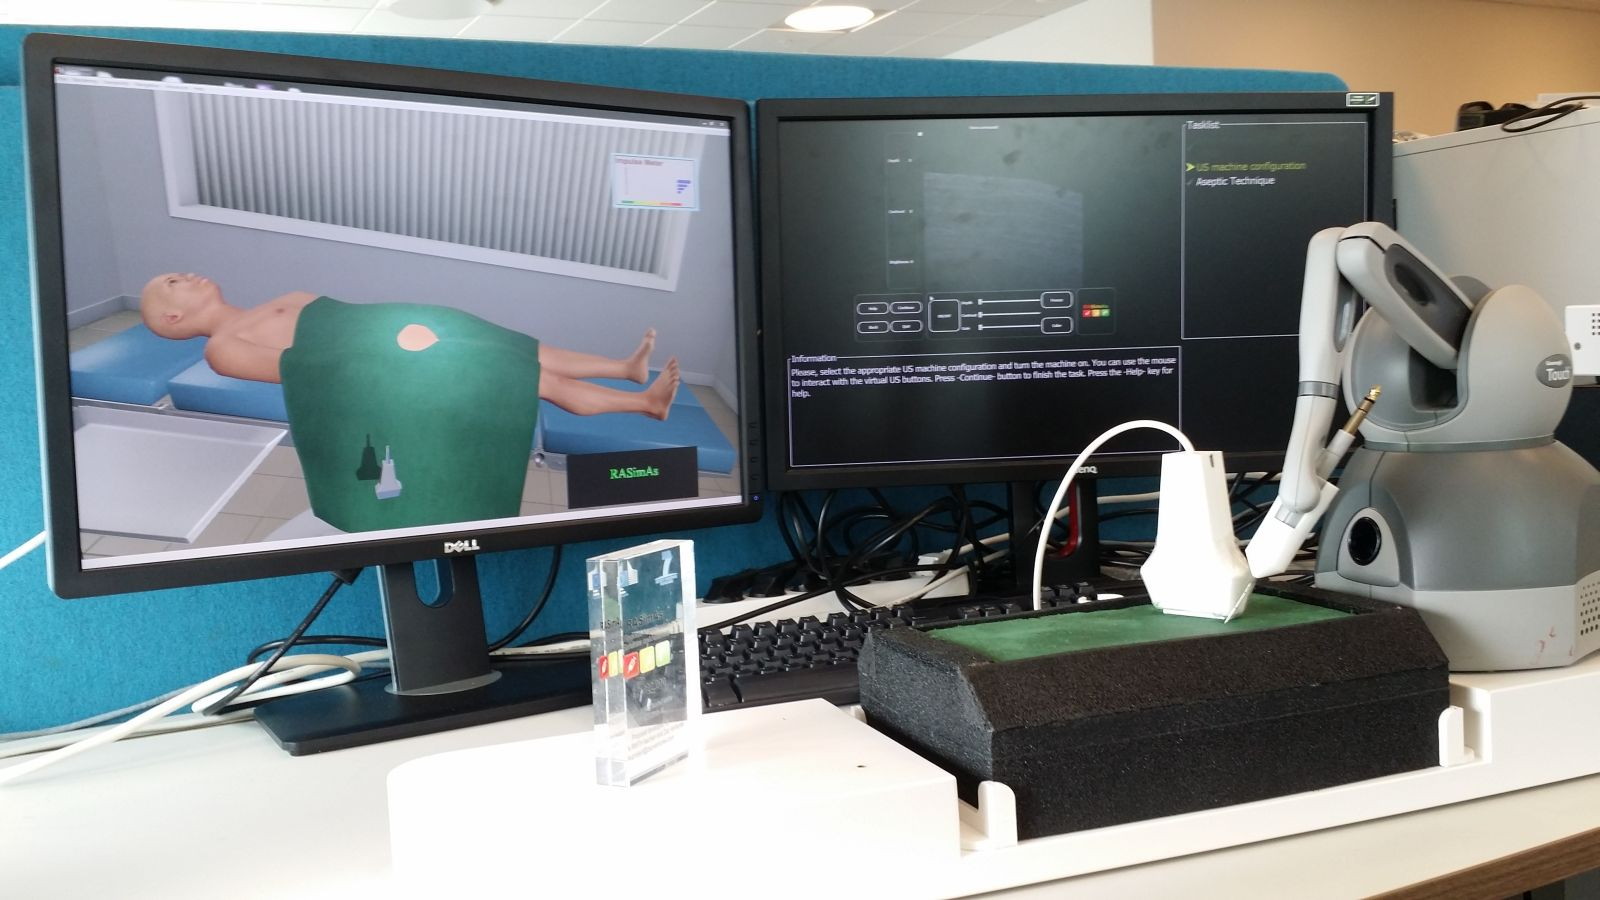
\includegraphics[width=1\textwidth]{IMG/sim3.jpg}
    \caption{\acs{RASim} \label{subfig:rasim}}
  \end{subfigure}%
  \begin{subfigure}[b]{0.5\linewidth}
    \centering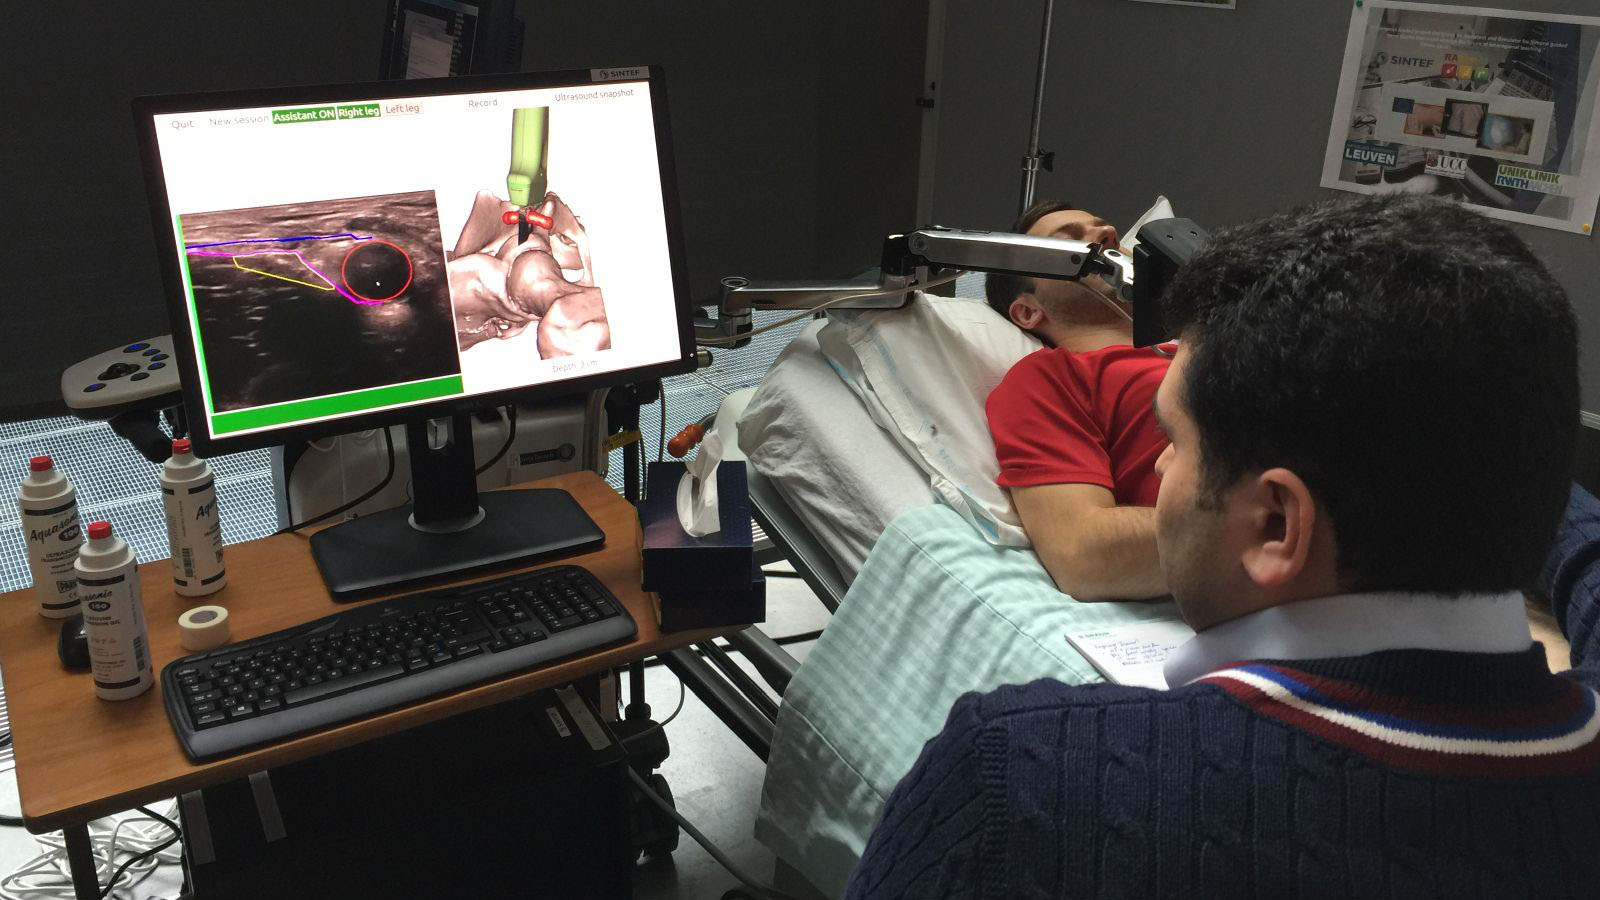
\includegraphics[width=1\textwidth]{IMG/raas.JPG}
    \caption{\acs{RAAs} \label{subfig:raas}}
  \end{subfigure}
  \caption{Imágenes que muestran los dos prototipos desarrollados en el contexto de \acs{RASimAs}.}
\end{figure}

%https://www.openanesthesia.org/regional-anesthesia-curriculum/
%http://rasimas.imib.rwth-aachen.de/member_area/documents_ma/Extra_Material/ISRA_Anaesthesia_Foundation_Course_Book_v1_to_print_for_ISRA_course_Oct_2_2014.pdf
%\todo{ Pon alguna cita, aquí y en el estado del arte. Por ejemplo, el CV de RA de Cork. Esto luego lo usaras en el courseware}

La \ac{RA} es un procedimiento mínimamente invasivo en el cual el médico administra un anestésico local en las proximidades del nervio que se desea bloquear \cite{CVraisra}. Esta técnica, frente a la anestesia general y si se practica adecuadamente, reduce: los efectos adversos sobre el paciente, su tiempo de recuperación y el coste de la intervención \cite{PMID:26695878}. La dificultad principal del procedimiento radica en liberar el bolo anestésico alrededor del nervio, sin tocarlo, evitando liberar la dosis en el torrente sanguíneo y confirmar que éste se ha extendido correctamente a su alrededor. Actualmente, existen dos técnicas para guiar la aguja hacia su objetivo: la estimulación eléctrica del nervio y el uso de imagen por \ac{US}. Aunque ambas técnicas pueden combinarse, la tendencia actual es abandonar la electroestimulación en favor del guiado por \ac{US}.

% \del{La \ac{RA} es un procedimiento médico dónde el \del{anestesiólogo}\new{anestesista!!!!!} administra anestésicos locales al paciente, a través de una aguja guiada por \ac{US} \todo{ojo hay otras formas de guiado. Tienes que ser muy preciso} en áreas cercanas a nervios específicos, produciendo una disminución de su actividad y ausencia del dolor. Esto posibilita la realización de cirugías sin necesidad de dormir al paciente completamente. De esta manera, se puede reducir el dolor postoperatorio, mejora la recuperación postoperatoria y se reduce el tiempo de hospitalización. De hecho, la anestesia regional se está imponiendo frente a la anestesia general debido a su menor coste e impacto en el paciente. \todo{cita}}
Sin embargo, esta técnica no es sencilla para los anestesistas que no están familiarizados con la ultrasonografía. Requiere tener una buena base teórica y práctica que permita proceder de manera segura. Hoy en día, está técnica se aprende principalmente practicándola sobre el paciente (\emph{by doing}), aunque existen otras técnicas como el uso de cadáveres \cite{Tsui2007} o \emph{fantomas}\footnote{Castellanización del término inglés Phantom.} \cite{phantomra}. Estas técnicas tienen claras limitaciones como: un alto coste,
la imposibilidad de repetir escenarios, el aprendizaje auto-guiado, 
que el usuario no se enfrente a una amplia variabilidad anatómica, etcétera.
%\borrar{enfrentar al usuario a una amplia variabilidad anatómica, etc.}

En primer lugar, \ac{RAAs} es un sistema de guiado que superpone información adicional sobre la imagen de \ac{US}, ayudando al usuario a identificar distintas regiones de interés. El sistema dispone de un \ac{tracker} y de un módulo de análisis de imagen que ayudan al médico a reconocer la aguja, la trayectoria de esta y las estructuras anatómicas relevantes mientras se está realizando la operación. 
% \del{Respecto a el sistema de guiado \ac{RAAs} consiste en asistir al anestesiólogo durante el procedimiento de \ac{RA}. Este sistema consta de unos dispositivos de seguimiento incorporados en la aguja y en la sonda del \ac{US}, de tal manera que con la información de seguimiento y la imagen de \ac{US}, el asistente proporcionará retroalimentación de inmediato que ayudará al médico a interpretar la imagen de \ac{US} de la anatomía del paciente.}


%\todo{Rehaz este parrafo. 1. No entiendo porque solo destacas 2 modulos del sistema el haptico y el fantoma. No has hablado del curseware, de las métricas del modo guiado. Del modulo físico, del modulo de ultrasonidos. Estructuralo todo en partes Hw y Sw y detallalas todas. } 
%
\ac{RASim} es un simulador médico que recrea un entorno de \ac{RA} donde el usuario puede entrenar el procedimiento. El usuario se sitúa en frente de la mesa de trabajo donde podrá encontrar: un maniquí y los dispositivos de \ac{E/S}.
El usuario interacciona con el sistema a través de una sonda de \ac{US}, con un \ac{tracker} magnético incorporado, y una aguja, acoplada a un dispositivo háptico. Estos dispositivos permiten al sistema seguir los movimientos del operador y proporcionar una respuesta háptica (en el caso de la aguja).
El usuario puede seguir el avance del procedimiento gracias a dos pantallas. En una, se muestra una vista virtual de la sala de operaciones  y, en la otra, se muestra la interfaz de la \ac{Courseware}\footnote{Software diseñado para fines educativos que sirve como ayuda o refuerzo del contenido.} con la imagen simulada de \ac{US}.
%
Así mismo, el simulador se compone de varios módulos software:
\begin{itemize}
    \item Módulo de respuesta háptica para la aguja.
    \item Simulación física entre los tejidos y los instrumentos médicos.
    \item Módulo de simulación de imágenes de \ac{US}.
    \item Renderizado de la escena virtual.
    \item Plataforma de autoevaluación y aprendizaje (\acs{Courseware}).
\end{itemize}

Es importante destacar que el módulo \ac{Courseware} es el que convierte al simulador en una plataforma de entrenamiento. Este software dirige al usuario a través del procedimiento mientras coordina todos los módulos del simulador en función del tipo de entrenamiento.  
%
El simulador permite practicar el procedimiento completo en un entorno seguro, además de mejorar sus habilidades cognitivas y no cognitivas gracias a la realimentación que proporciona el sistema.

Con el objetivo de enfrentar a los médicos a distintos escenarios que representen una variabilidad anatómica significativa, en el proyecto \ac{RASimAs} se ha propuesto desarrollar un entorno integrado de generación de pacientes virtuales (en inglés: \ac{ITGVPH}) con el que generar una base de datos de pacientes virtuales  que  podrán ser utilizados en \ac{RASim}. 
%
Esta herramienta genera \ac{VPH}, a partir del registro de un modelo virtual con imágenes de pacientes reales.
También es capaz de cambiar la postura inicial del paciente virtual a la posición requerida por el procedimiento y generar el comportamiento mecánico de los tejidos necesarios para su simulación física. Cabe destacar que los pacientes virtuales generados por esta herramienta no se corresponden con datos de pacientes reales, sino con variedades anatómicas representativas.
%\new{Por otra parte, este mismo sistema puede ser usado como plataforma de entrenamiento autoguiado en la que el usuario puede practicar el procedimiento gracias a la retroalimentación que el sistema proporciona.}

%Se ha diseñado una mesa de trabajo donde el usuario interacciona con el sistema. En ella, se encuentran dos pantallas que sirve para proporcionar información visual al usuario. En una de ellas se puede visualizar una vista de la sala de operaciones virtual y en otra, se muestra la vista del software de entrenamiento junto con la imagen simulada de \ac{US}. En la mesa de trabajo, el usuario maneja una sonda de \ac{US}, con un \ac{tracker} magnético incorporado, y una aguja, acoplada a un dispositivo háptico, que permite al sistema el seguimiento de los movimientos del usuario. El simulador es capaz de simular la interacción y deformación de los instrumentos y tejidos, y generar una imagen de \ac{US}. El \ac{Courseware} es el encargado de dirigir al usuario a través del procedimiento y gestionar todos los modulos del simulador. 

%\todo{tienes que restructurar toda la información de RASim. 1. Objetivos (no uses la palabra objetivos todo el rato):variabilidad anatómica gran base de datos de pacientes, aprendizaje autónomo, autoevalucaion (no digas evaluación es demasiado ambicioso). 2. Modulos Hw y Sw. Importante: no me lo vuelvas a pasar hasta que lo hayas leído 3 veces. No puedo dedicar tanto tiempo a cada capítulo. Ojo Con las afirmaciones como modulo realista (si no esta evaluado, no lo sabes. Por otro lado, el módulo haptico es una mierda). }
%El objetivo de este simulador es que el usuario pueda aprender el procedimiento completo en un entorno seguro y además pueda practicar sus habilidades cognitivas y no cognitivas en el sistema. 
%\todo{demasiado ambicioso}
%de las capacidades de los profesionales, gracias a los dispositivos hápticos y a la simulación física la cual es capaz de recoger parámetros de rendimiento más allá de valoraciones subjetivas que podría tener un supervisor.\todo{No dices nada de autoguiado, ni de autoevaluación.}






%\subsection{Contribuciones al proyecto RASimAs}
%\label{intro:context}

\begin{figure}
    \centering
    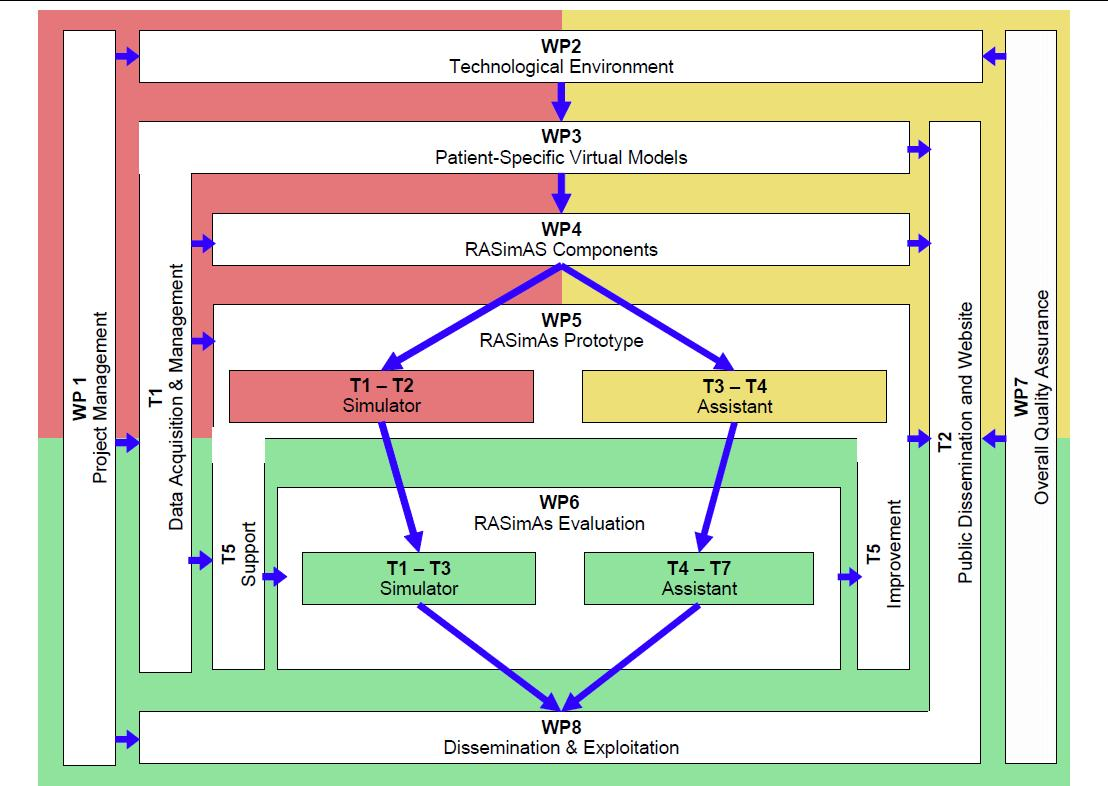
\includegraphics[width=0.95\textwidth]{IMG/wp_overview.jpg}
    \caption{División y organización de los \acl{WP} de \acs{RASimAs}.}
    \label{fig:wp_rasimas}
\end{figure}

El proyecto \ac{RASimAs} se organiza en los ocho \ac{WP} que se pueden observar en la figura \ref{fig:wp_rasimas}. Los \ac{WP} 1, 7 y 8 se encargarán de tareas de gestión: coordinación, control de calidad, diseminación de resultados y explotación de los prototipos. El \ac{WP} 2 desarrollará la plataforma donde se integrarán todos los módulos de software y datos generados de los siguientes paquetes. En los \ac{WP} 3 y 4 se desarrollarán los componentes necesarios de los dos prototipos que se integrarán en el \ac{WP} 5. Por último, el \ac{WP} 6 se encarga de la evaluación clínica tanto del prototipo de \ac{RASim} como del \ac{RAAs}. 

En la sección \ref{art:rasimas} , se introducirán los \ac{WP} 3, 4 y 5 y las tareas en las que ha contribuido de manera activa la \ac{URJC}, en las cuales se encuadra la mayor parte de la investigación realizada en esta tesis.


\subsection{Colaboración con \acl{Bangor}}
%\todo{Aaron, se que soy un pesado, pero cuando te digo que pienses cada frase me refiero a esto. El motivo por el que las colaboraciones entre miembros del proyecto van más allá de las tareas del mismo, NO es que trabajen distintas instituciones, SINO que estos proyectos permiten conocer de forma más próxima el trabajo que se está realizando en otros laboratorios }
%\todo{Para nada considero que seas pesado, al revés, el conformista soy yo...}
%
Una de las ventajas que tienen los proyectos internacionales de esta índole es que mejoran la visibilidad del trabajo realizado por los miembros del consorcio, fomentando colaboraciones entre socios más allá del ámbito del proyecto.
%
En el caso de este trabajo de tesis, \ac{RASimAs} proporcionó la oportunidad de conocer en profundidad el trabajo del  Dr. Franck P. Vidal, miembro de la \emph{School of Computer Science} de \acl{Bangor}, en el campo de la simulación de generación de imágenes médicas de rayos X en tiempo real \cite{villard2014interventional}. El Dr. Frank P. Vidal es el responsable de la librería \emph{gVirtualXRay} \cite{gVirtualXRay}.
%
A partir de esta tecnología y la herramienta de posicionamiento de pacientes, creada en el contexto del proyecto \ac{RASimAs}, se propuso desarrollar un simulador de radiología diagnóstica en el que seguir evaluando la viabilidad de los algoritmos propuestos en este trabajo.
%que utilizará los dos módulos para permitir a un usuario practicar el posicionamiento de un paciente por parte de un radiólogo.

La radiología es una especialidad de diagnóstico por imagen que utiliza la tecnología de los rayos X. Debido a la peligrosidad de una exposición prolongada a estos rayos, un simulador que permita al radiólogo entrenar de manera segura y que pudiera ser utilizado sin restricciones de tiempo, sería de gran utilidad en el campo.
Como resultado de esta colaboración, se han podido realizar dos estancias del autor de esta tesis en la \acl{Bangor}. 

%1. El proyecto Rasimas nos da la oportunidad de trabajar con miembros de la universidad de Bangor y conocer su trabajo.2. Frank School of Health Sciences y el otro School of Computer Science and Electronic Engineering3. Trabajan en radiologia (prescisa un poco dar mas detalles. Habla de sus publicaciones)4. Se plantea adpartar y extender las técnicas desarrolladas en el contexto de RaSimasç5. La colaboración se articula en dos estancias.}





